\documentclass[a4paper]{article}

\setlength{\parindent}{0pt}
\setlength{\parskip}{1em}

\pagestyle{headings}

\usepackage{amssymb}
\usepackage{amsmath}
\usepackage{amsthm}
\usepackage{mathtools}
\usepackage{graphicx}
\usepackage{hyperref}
\usepackage{color}
\usepackage{microtype}
\usepackage{tikz}
\usepackage{pgfplots}
\usepackage{pgfplotstable}

\newcommand{\N}{\mathbb{N}}
\newcommand{\Q}{\mathbb{Q}}
\newcommand{\Z}{\mathbb{Z}}
\newcommand{\R}{\mathbb{R}}
\newcommand{\C}{\mathbb{C}}
\newcommand{\D}{\mathcal{D}}
\renewcommand{\S}{\mathcal{S}}
\renewcommand{\P}{\mathbb{P}}
\newcommand{\F}{\mathbb{F}}
\newcommand{\E}{\mathbb{E}}
\newcommand{\bra}{\langle}
\newcommand{\ket}{\rangle}


\graphicspath{{Image/}}

\hypersetup{
    colorlinks=true,
    linktoc=all,
    linkcolor=blue
}

\theoremstyle{definition}
\newtheorem*{axiom}{Axiom}
\newtheorem*{claim}{Claim}
\newtheorem*{conv}{Convention}
\newtheorem*{coro}{Corollary}
\newtheorem*{defi}{Definition}
\newtheorem*{eg}{Example}
\newtheorem*{lemma}{Lemma}
\newtheorem*{notation}{Notation}
\newtheorem*{prob}{Problem}
\newtheorem*{post}{Postulate}
\newtheorem*{prop}{Proposition}
\newtheorem*{rem}{Remark}
\newtheorem*{thm}{Theorem}

\DeclareMathOperator{\vdiv}{div}
\DeclareMathOperator{\grad}{grad}
\DeclareMathOperator{\curl}{curl}
\DeclareMathOperator{\Ann}{Ann}
\DeclareMathOperator{\Fit}{Fit}
\DeclareMathOperator{\Diag}{Diag}
\DeclareMathOperator{\tr}{tr}
\DeclareMathOperator{\im}{im}
\DeclareMathOperator{\Mat}{Mat}
\DeclareMathOperator{\Log}{Log}
\DeclareMathOperator{\Isom}{Isom}
\DeclareMathOperator{\Mesh}{Mesh}
\DeclareMathOperator{\Sym}{Sym}
\DeclareMathOperator{\Aut}{Aut}
\DeclareMathOperator{\cosech}{cosech}
\DeclareMathOperator{\Card}{Card}
\DeclareMathOperator{\Gal}{Gal}


\setcounter{section}{-1}

\begin{document}

\title{Combinatorics}

\maketitle

\newpage

\tableofcontents

\newpage

\section{Introduction}

In this course we'll discuss three main aspects:\\
$\bullet$ Set systems;\\
$\bullet$ Isoperimetric Inequalities;\\
$\bullet$ Projections (combinatorics in continuous settings).

References:\\
\emph{Combinatorics}, Bocabas, Cambridge University Press, 1986 (chapter 1,2);\\
\emph{Combinatorics and finite sets}, Anderson, Oxford University Press, 1987 (chapter 1).

\newpage

\section{Set Systems}

Let $X$ be a set. A \emph{set system} on $X$ (or family of subsets of $X$) is a family $\mathcal{A} \subset \P(X)$.\\
For example, we define $X^{(r)} = \{A \subset X: |A| = r\}$.

Unless otherwise stated, $X=[n] = \{1,2,...,n\}$. For example, $|X^{(r)}| = {n \choose r}$ (assume finiteness). So $[4]^{(2)} = \{12,13,14,23,24,34\}$.

We often make $\P(x)$ into a graph, called $Q_n$, by joining $A$ to $B$ if $|A \triangle B| = 1$ (symmetric difference).

(examples of $Q_3,Q_n$)

If we identify a set $A \subset X$ with a 0-1 sequence of length $n$ via $A \leftrightarrow 1_A$ (characteristic function), then $Q_3$ acn be thought of as a cube. In general, $Q_n$ is an $n$-dimensional cube (hypercube/discretecube/$n$-cube/...).

\subsection{Chains and antichains}
A family $\mathcal{A} \subset \P(X)$ is a \emph{chain} if $\forall A,B \in \mathcal{A}, A \subset B$ or $B \subset A$. It is an antichain if $\forall A \neq B \in \mathcal{A}$, $A \not\in B$.

Obviously the maximum size of a chain in $X$ is $n+1$.

For antichains, we can take $X^{\lfloor\frac{n}{2}\rfloor}$, which has size ${n \choose {\lfloor n/2 \rfloor}}$. The result is that wee can't beat this, but the proof is not trivial.

---Lecture 2---

No lecture this thursday (11 Oct 2018)!

Idea: inspired by \emph{each chain meets each level $X^{(r)}$ in at most one place} -- try to decompose $Q_n$ into chains.

\begin{thm} (Sperner's Lemma)\\
    Let $A \subset \P(X)$ be an antichain. Then $|A| \leq {n \choose {\lfloor n/2 \rfloor}}$.
    \begin{proof}
        It's sufficient to partition $\P(X)$ into that many chains (since an anti-chain and a chain can have at most one common vertex).\\
        For this, it's sufficient to show:\\
        $\bullet$ $\forall r < n/2$, there exists a matching (set of disjoint edges) from $X^{(r)}$ to $X^{(r+1)}$;\\
        $\bullet$ $\forall r > n/2$, there exists a matching from $X^{(r)}$ to $X^{(r-1)}$.\\
        (Then put these matchings together to form chains, each passing through $X^{(\lfloor n/2 \rfloor)})$, so the result.\\
        By taking complements it's sufficient to prove (i).\\
        Consider subgraph of $Q_n$ spanned by $X^{(r)} \cup X^{(r+1)}$ which is bipartite. For any $B \subset X^{(r)}$, we have:\\
        $\bullet$ number of $B-\P(B)$ edges = $|B| (n-r)$; (each point in $X^{(r)}$ has degree $(n-r)$)\\
        $\bullet$ number of $B-\P(B)$ edges $\leq$ $|\P(B)|(r+1)$. (each point in $X^{(r+1)})$ has degree $r+1$)\\
        Thus $|\P(B)| \geq |B| \frac{n-r}{r+1} \geq |B|$, as $r < n/2$.\\
        Hence by Hall's theorem there exists a matching.
    \end{proof}
\end{thm}

\begin{rem}
    $\bullet$ 1. ${n \choose {\lfloor n/2 \rfloor}}$ is achievable by just taking $X^{(\lfloor n/2 \rfloor)}$.\\
    $\bullet$ 2. This proof says nothing about extremal cases: which antichains have size ${n \choose {\lfloor n/2 \rfloor}}$?
\end{rem}

Aim: For $\mathcal{A}$ an antichain, $\sum_{r=0}^n \frac{|\mathcal{A} \cap X^{(r)}|}{{n \choose r}} \leq 1$. Note that this trivally implies Sperner's lemma.

Let $\mathcal{A} \subset X^{(r)}$ for some $1 \leq r \leq n$. The \emph{shadow} or \emph{lower shadow} of $\mathcal{A}$ is
\begin{equation*}
    \begin{aligned}
        \partial A = \partial^- A = \{A-\{i\}:A \in \mathcal{A},i \in A\}
    \end{aligned}
\end{equation*}
So $\partial A \subset X^{(r-1)}$.

For example, if $\mathcal{A} = \{123,124,134,135\} \subset X^{(3)}$, then $\partial A =\{12,13,23,14,24,34,15,35\} \subset X^{(2)}$.

\begin{lemma} (Local LYM)\\
    Let $\mathcal{A} \subset X^{(r)}$, $1 \leq r \leq n$. Then 
    \begin{equation*}
        \begin{aligned}
            \frac{|\partial \mathcal{A}|}{{n \choose {r-1}}} \geq \frac{|\mathcal{A}|}{{n \choose r}}
        \end{aligned}
    \end{equation*}
    (\emph{the fraction of the layer occupied increases when we take the shadow}.)
    \begin{proof}
        $\bullet$ Number of $\mathcal{A}-\partial\mathcal{A}$ edges (in $Q_n$) = $r|\mathcal{A}|$ (counting from above);\\
        $\bullet$ Number of $\mathcal{A}-\partial\mathcal{A}$ edges $\leq$ $(n-r+1)|\partial \mathcal{A}|$ (counting from below).\\
        So
        \begin{equation*}
        \begin{aligned}
            \frac{|\partial \mathcal{A}|}{|\mathcal{A}|} \geq \frac{r}{n-r+1}
        \end{aligned}
        \end{equation*}
        However RHS is the ratio of size between the two layers.
    \end{proof}
\end{lemma}
Let's consider when is equality achieved in local LYM. we need $A-\{i\} \cup \{j\} \in \mathcal{A}$ $\forall A \in \mathcal{A}, i \in A, j \not\in A$.\\
Hence $\mathcal{A} = X^{(r)}$ or $\phi$.

\begin{thm} (Lubell-Yamamoto-Meshalkin inequality)\\
    Let $\mathcal{A} \subset \P(X)$ be an antichain. Then $\sum_{r=0}^n \frac{|\mathcal{A} \cap X^{(r)}|}{{n \choose r}} \leq 1$.
    \begin{proof} (1, \emph{Bubble down with local LYM})\\
        Let's start with $X^{(r)}$. Write $\mathcal{A}_r$ for $\mathcal{A} \cap X^{(r)}$.\\
        We have $\frac{|\mathcal{A}_n|}{{n\choose n}} \leq 1$ (trivially).\\
        Also, $\partial \mathcal{A}_n$ and $\mathcal{A}_{n-1}$ are disjoint (as $\mathcal{A}$ is an antichain). So 
        \begin{equation*}
        \begin{aligned}
            \frac{|\partial \mathcal{A}_n|}{{n \choose {n-1}}} + \frac{|\mathcal{A}_{n-1}|}{{n \choose {n-1}}} = \frac{|\partial \mathcal{A}_n \cup \mathcal{A}_{n-1}|}{{n \choose {n-1}}} \leq 1
        \end{aligned}
        \end{equation*}
        So
        \begin{equation*}
        \begin{aligned}
            \frac{|\mathcal{A}_n|}{{n \choose n}} + \frac{|\mathcal{A}_{n-1}|}{{n \choose {n-1}}} \leq 1
        \end{aligned}
        \end{equation*}
        by local LYM. Note that we have successfully expanded LHS to two terms.\\
        Also, $\partial (\partial \mathcal{A}_n \cup \mathcal{A}_{n-1})$ is disjoint from $\mathcal{A}_{n-2}$ again since $\mathcal{A}$ is an antichain. So 
        \begin{equation*}
            \begin{aligned}
                \frac{|\partial(\partial \mathcal{A}_n \cup \mathcal{A}_{n-1})|}{{n \choose {n-2}}} + \frac{|\mathcal{A}_{n-2}|}{{n \choose {n-2}}} \leq 1
            \end{aligned}
        \end{equation*}
        So
        \begin{equation*}
            \begin{aligned}
                \frac{|\partial \mathcal{A}_n \cup \mathcal{A}_{n-1}|}{{n \choose {n-1}}} + \frac{|\mathcal{A}_{n-2}|}{{n \choose {n-2}}} \leq 1
            \end{aligned}
        \end{equation*}
        So
        \begin{equation*}
            \begin{aligned}
                \frac{|\mathcal{A}_n|}{{n \choose {n}}} + \frac{|\mathcal{A}_{n-1}|}{{n \choose {n-1}}} + \frac{|\mathcal{A}_{n-2}|}{{n \choose {n-2}}} \leq 1
            \end{aligned}
        \end{equation*}
        Keep going and we obtain the desired result.
    \end{proof}
\end{thm}

When is equality achieved in LYM? We must have equality in each use of local LYM, so the first $r$ with $\mathcal{A}_r \neq \phi$ must have $\mathcal{A}_r = X^{(r)}$, i.e. $\mathcal{A} = X^{(r)}$.

Hence equality in Sperner's lemma is only achieved when $\mathcal{A} = X^{\lfloor n/2 \rfloor}$ for $n$ even, or also $X^{\lceil n/2 \rceil}$ when $n$ is odd.

---Lecture 3---

Now let's look at another proof to LYM inequality:
\begin{proof} (2) \\
    Choose, uniformly at random, a maximal chain $\mathcal{C}$ (i.e. $C_0 \subset C_1 \subset ... \subset C_n$ with $|C_i| =i \forall i$). For a given $r$-set $A$ (which is just one vertex in our graph, if you rememeber what our vertices mean), $\P(A \in \mathcal{C}) = \frac{1}{{n \choose r}}$. So $\P(\mathcal{A}_r \text{ meets } \mathcal{C}) = \frac{|\mathcal{A}_r|}{{n \choose r}}$ (events are disjoint).\\
    So $\P(\mathcal{A} \text{ meets } \mathcal{C}) = \sum_{r=0}^n \frac{|\mathcal{A}_r|}{{n \choose r}}$, but that can be no greater than 1.
\end{proof}

\begin{rem}
    Equivalently, we could also do counting: the number of maximal chains is $n!$, and the number containing a given $r$-sets is $r!(n-r)!$. So we get $\sum|\mathcal{A}_r|r!(n-r)! \leq n!$ -- we can rearrange to get LYM as well.
\end{rem}

\subsection{Shadows}
For $\mathcal{A} \subset X^{(r)}$, we know $|\partial A| \geq |\mathcal{A}| \frac{r}{n-r+1}$, but equality is rare (only for extreme cases $\phi$ or $X^{(r)}$).\\
It then comes to our interests how we should choose $\mathcal{A} \subset X^{(r)}$ to minimize $|\partial A|$ for any fixed given $|\mathcal{A}|$, which is in some sense, how \emph{tightly} can we \emph{pack} some $r$-sets.\\
One trivial observation: if $|\mathcal{A}| = {k \choose r}$, it's believable that we would take $\mathcal{A} = [k]^{(r)}$ which gives $\partial A =[k]^{(r-1)}$.\\
What if ${k \choose r} < |\mathcal{A}| < {{k+1} \choose r}$? Naturally we expect to take $[k]^{(r)}$ with some others. For example, if $\mathcal{A} \subset X^{(3)}$ with $|\mathcal{A}| = {7 \choose 3} + {4 \choose 2}$, we'd take $\mathcal{A} = [7]^{(3)} \cup \{A \cup \{8\}: A \in [4]^{(2)}\}$. If we play around with this method and look at the $\mathcal{A}$ we choose each time, we note that there seems to be some order in $X^{(r)}$ that, whenever we are given $|\mathcal{A}| = m$, we should just pick the first $m$ $r-$sets in that order.

\subsubsection{Total orderings on $X^{(r)}$}
\begin{defi}
Given $A,B \in X^{(r)}$, say $A = a_1...a_r,B=b_1...b_r$ where $a_1<...<a_r$ and same for $b_i$. We say $A<B$ in the \emph{lexicographic} (or \emph{lex}) order, if for some $i$ we have $a_i < b_i$ and $a_j = b_j$ $\forall j < i$. Equivalently, $a_i<b_i$, where $i=\min\{j: a_j \neq b_j\}$ (use small numbers).\\
Given $A<B$ in the \emph{colexicographic} or \emph{colex} order if, for some $i$ have $a_i<b_i$, and $a_j=b_j$ $\forall j>i$. Equivalently, $a_i < b_i$ where $i = \max\{j:a_j \neq b_j\}$ (avoid large numbers). State it in a cooler way, $A<B$ if $\sum_{i \in A} 2^i < \sum_{i \in B} 2^i$.\\
(some useless examples)
\end{defi}

Note: in colex, $[k]^{(r)}$ is an initial segment of $[k+1]^{(r)}$, so we could view colex as an enumeration of $\N^{(r)}$d (but not for lex -- we'll have to know the size of the ground set first before deciding what's coming next)!\\
Indeed, the colex order is what we need to use for the shadow problem, i.e. if $\mathcal{A} \subset X^{(r)}$, and $\mathcal{C} \subset X^{(r)}$ is the first $|\mathcal{A}|$ $r$-sets in colex, then $|\partial \mathcal{A}| \geq |\partial \mathcal{C}|$ (\href{https://en.wikipedia.org/wiki/Kruskal%E2%80%93Katona_theorem}{Kruskal-Katona theorem}). In particular, $|\mathcal{A}| = {k \choose r} \implies |\partial \mathcal{A}| \geq {k \choose {r-1}}$).

\subsubsection{Compressions}
Idea: we want to \emph{replace} $\mathcal{A} \subset X^{(r)}$ with some $A' \subset X^{(r)}$, such that\\
(i) $|\mathcal{A}'| = |\mathcal{A}|$;\\
(ii) $|\partial \mathcal{A}'| \leq |\partial \mathcal{A}|$;\\
(iii) $\mathcal{A}'$ \emph{looks more like $\mathcal{C}$} then $\mathcal{A}$ did.

Ideally, we'd compress $\mathcal{A} \to \mathcal{A}' \to \mathcal{A}'' \to ... \to \mathcal{B}$ where either $\mathcal{B} = \mathcal{C}$, or $\mathcal{B}$ is so similar to $\mathcal{C}$ that we can see directly that $|\partial \mathcal{B}| \geq |\partial \mathcal{C}|$.

---Lecture 4---

We'll follow two general ideas to obtain our desired result:

$\bullet$ \emph{Colex prefers 1 to 2} inspires:\\
For $1 \leq i < j \leq n$, the $ij-$compression $C_{ij}$ is defined by: for $A \subset X$,
\begin{equation*}
    \begin{aligned}
        C_{ij}(A) = \left\{
            \begin{array}{ll}
                A-j \cup i & \text{ if } j \in A, i \not\in A\\
                A & \text{ otherwise}
            \end{array}
        \right.
    \end{aligned}
\end{equation*}
and for $\mathcal{A} \subset \P(X)$, $C_{ij}(\mathcal{A}) = \{C_{ij}(A):A \in \mathcal{A}\} \cup \{A \in \mathcal{A}:C_{ij}(A) \in \mathcal{A}\}$.\\
Note that $|C_{ij}(\mathcal{A})| = |\mathcal{A}|$.

We say $\mathcal{A}$ is \emph{$ij$-compressed} if $C_{ij}(\mathcal{A}) = \mathcal{A}$.

\begin{prop} (4)\\
    Let $\mathcal{A} \subset X^{(r)}$, $1 \leq i < j \leq n$. Then $|\partial C_{ij}(\mathcal{A}) | \leq |\partial \mathcal{A}|$.\\
    (Shadow of a compressed set is no larger than that of the original.)
    \begin{proof}
        Write $\mathcal{A'}$ for $C_{ij}(\mathcal{A})$. We'll show that if $B \in \partial \mathcal{A}' - \partial A$, then $i \in B, j \not \in B$, and $B \cup j - i \in \partial \mathcal{A} - \partial{A'}$, then we are done since for each new elememt that we probably introduced, there's one element removed.\\
        We have $B \cup x \in \mathcal{A}'$ for some $x \not\in B$, and $B \cup x \not\in \mathcal{A}$ (as $B \not\in \partial \mathcal{A}$).\\
        Hence $i \in B \cup x$, $j \not\in B \cup x$, and $(B \cup x ) \cup j - i \in \mathcal{A}$. Note that $i \neq x$, since otherwise $B \cup j \in \mathcal{A}$.\\
        Certainly $B \cup j - i \in \partial \mathcal{A}$. Now we claim that $B \cup j - i \not\in \partial \mathcal{A}'$: suppose $(B \cup j - i) \cup y \in \mathcal{A}'$. We cannot have $y=i$ for else $B \cup j \in \mathcal{A}'$, then $B\cup j$ have to be in $\mathcal{A}$ by definition of compression; but that's not allowed.\\
        Thus $j \in (B\cup j - i) \cup y$, $i \not\in (B \cup j - i) \cup y$. So $(B \cup j - i) \cup y \in \mathcal{A}$, so $B \cup y \in \mathcal{A}$ by definition of compression; but that's similarly a contraditction.
    \end{proof}
\end{prop}

\begin{rem}
    We've actually shown that $\partial C_{ij}(\mathcal{A}) \subset C_{ij}(\partial \mathcal{A})$.
\end{rem}

We say $\mathcal{A} \subset X^{(r)}$ is \emph{left-compressed} if $C_{ij}(\mathcal{A}) = \mathcal{A}$ $\forall i < j$.

\begin{prop}
    Let $\mathcal{A} \subset X^{(r)}$. Then there is a left-compressed $\mathcal{B} \in X^{(r)}$ with $|\mathcal{B}| = |\mathcal{A}|$, and $|\partial \mathcal{B}| \leq |\partial \mathcal{A}|$.
    \begin{proof}
        Among all $\mathcal{B} \subset X^{(r)}$ with $|\mathcal{B}| = |\mathcal{A}|$ and $|\partial \mathcal{B}| \leq |\partial \mathcal{A}|$, choose one with $\sum_{A \in \mathcal{B}} \sum_{x \in A} x$ minimal.\\
        Then $\mathcal{B}$ is left-compressed, else we can compress it to reduce the above sum.
    \end{proof}
\end{prop}

Note: we can also apply $C_{ij}$ repeatedly -- this must terminate (by counting on the above sum). In fact, we can apply each $C_{ij}$ at most once if we choose a sensible order.

Certainly, initial segments of colex are left-compressed. However the converse can be very false (consider $\{123,124,125,126,127\}$).

$\bullet$ \emph{Colex prefers 23 to 14} inspires:\\
For $U,V \subset X$ with $|U| = |V|$, and $U \cap V = \phi$, the $UV$-compression $C_{UV}$ is defined by: for $A \subset X$,
\begin{equation*}
    \begin{aligned}
        C_{UV}(A) = \left\{
            \begin{array}{ll}
                A\cup U - V & \text{ if } V \subset A, U \cap A = \phi\\
                A & \text{ otherwise}
            \end{array}
        \right.
    \end{aligned}
\end{equation*}
and for $\mathcal{A} \subset X^{(r)}$, $C_{UV}(A) = \{C_{UV}(A):A \in \mathcal{A}\} \cup \{A \in \mathcal{A}: C_{UV}(A)\in \mathcal{A}\}$.

Note that also the two sets have equal size. We say $\mathcal{A}$ is \emph{$UV$-compressed} if $C_{UV}(\mathcal{A}) = \mathcal{A}$.

Sadly $C_{UV}$ doesn't necessarily decrease the shadow.

However, it turns out to be fine if we have done the smaller ones.

\begin{prop}
    Let $\mathcal{A} \subset X^{(r)}$ and $U,V \subset X$ with $|U|=|V|$ and $U \cap V = \phi$. Suppose that\\
    (*) $\forall x \in U, \exists y \in V$ s.t. $\mathcal{A}$ is $(U-x,V-y)$-compressed.\\
    Then $|\partial C_{UV}(\mathcal{A})|\leq |\partial \mathcal{A}|$.
    \begin{proof}
        Write $\mathcal{A}'$ for $C_{UV}(\mathcal{A})$.\\
        Given $B \in \partial \mathcal{A}' - \partial \mathcal{A}$, we'll show that $U \cup B, V \cap P = \phi$, and $B \cup V - U \in \partial \mathcal{A} - \partial \mathcal{A}'$ (then we are done similar to the proof above).\\

---Lecture 5---

        We have $B \cup x \in \mathcal{A}'$ for some $x \not\in B$, with $B \cup x \not\in \mathcal{A}$.\\
        So $U \subset B \cup x$, $V \cap (B \cup x) = \phi$,and $(B \cup x) \cup V - U \in \mathcal{A}$.\\
        Thus certainly $V \cap B = \phi$.\\
        If $x \in U$: We have $\mathcal{A}$ is $(U-x,V-y)$ compressed for some $y \in V$. So from $(B \cup x) \cup V - U \in \mathcal{A}$, we obtain $B \cup y \in \mathcal{A}$, contradicting $B \not\in \partial \mathcal{A}$.\\
        Hence $x \not\in U$, and so $U \subset B$.\\
        Lastly, $B \cup V - U \in \partial \mathcal{A}$ as $(B \cup x) \cup V - U \in \mathcal{A}$ (so the first is in the shadow by removing $x$);\\
        Suppose $B \cup V- \in \partial \mathcal{A}'$. Then $(B \cup V - U) \cup w \in \mathcal{A}'$ for some $w$. If $w \not\in U$, then $V \subset (B \cup V - U) \cup w$, and $U \cap (B\cup V-U) \cup w = \phi$, so from $(B\cup V - U) \cup w \in \mathcal{A}'$ we conclude that both $(B-V-U) \cup W \in \mathcal{A}$, and $B \cup w \in \mathcal{A}$; however then $B \in \partial \mathcal{A}$, contradiction.\\
        Otherwise, if $w \in U$, we have $\mathcal{A}$ is $(U-w,V-z)$-compressed for some $z \in V$ by our assumption. Now from $(B \cup V-U) \cup w \in\mathcal{A}$, since it is in $\mathcal{A}'$ and contains $V$ so we could not have moved by compression. So we get $B \cup z \in \mathcal{A}$, but then $B \in \partial \mathcal{A}$; contradiction.
    \end{proof}
\end{prop}

With this tool, we can finally begin the proof of:
\begin{thm} (7, Kruskal-Katona)\\
    Let $\mathcal{A} \subset X^{(r)}$ $(1 \leq r \leq n)$, and let $\mathcal{C}$ be the initial segment of colex on $X^{(r)}$ with $|\mathcal{C}| = |\mathcal{A}|$. Then $|\partial \mathcal{A}| \geq |\partial \mathcal{C}|$.\\
    In particular, if $|\mathcal{A}| = {k \choose r}$, then $|\partial \mathcal{A}| \geq {k \choose {r-1}}$.
    \begin{proof}
        Let $\Gamma = \{(U,V): U,V \subset X, |U| = |V| > 0, U \cap V = \phi, \max U < \max V\}$.\\
        Define a sequence of set systems $\mathcal{A}_0,\mathcal{A}_1,...$ in $X^{(r)}$ as follows:\\
        Let $\mathcal{A}_0 = \mathcal{A}$. Having defined $\mathcal{A}_{k_1}$, if $\mathcal{A})k$ is $(U,V)-$compressed $\forall (U,V) \in \Gamma$, then stop the sequence with $\mathcal{A}_k$. If not, choose $(U,V) \in \Gamma$ s.t. $\mathcal{A}_k$ \emph{not} $(U,V)$-compressed, with $|U|$ minimal. Set $\mathcal{A}_{k+1} = C_{UV}(\mathcal{A}_k)$.\\
        Note that $\forall x \in U$, we have $(U-x,V-y) \in \Gamma \cup \{(\phi,\phi)\}$ for $y = \min V$. So by proposition 6, $|\partial \mathcal{A}_{k+1}| \leq |\partial \mathcal{A}_k|$. Continue.\\
        This sequence must terminate, as, for example, $\sum){A \in \mathcal{A}_k} \sum_{i \in A} 2^i$ is decreasing in $k$ (not important, just something that is monotonically decreasing).\\
        The final sysem $\mathcal{B} = \mathcal{A}_k$ satisfies $|\mathcal{B}| = |\mathcal{A}|$, and $|\partial \mathcal{B}| \leq |\partial \mathcal{A}|$, and is $(U,V)$-compressed for every $(U,V) \in \Gamma$.\\
        Now we claim $\mathcal{B} = \mathcal{C}$: suppose otherwise, that $\mathcal{B}$ is not an initial segment of colex. Then $\exists A < B$ in colex with $A \not\in \mathcal{B}$ and $B \in \mathcal{B}$.\\
        But then $U = A-B$ and $V=B-A$. We have $(U,V) \in \Gamma$, and $C_{UV}(B) = A$, so $\mathcal{B}$ is not $(U,V)$-compressed. Contradiction.
    \end{proof}
\end{thm}

\begin{rem}
    1. Equivalently: if $\mathcal{A} \subset X^{(r)}$ with $|\mathcal{A}| = {k_r \choose r} + {k_{r-1} \choose {r-1}} + ... + {k_s \choose s}$, where $k_r>k_{r-1}>...>k_s$ and $s>0$. Then $|\partial \mathcal{A}| \geq {k_r \choose {r-1}} + ... +{k_s \choose {s-1}}$ (Nice to know, but this is not important).\\
    2. In proof of K-K theorem we only used the above proposition 6 but not the simplfied $ij$-compression case; but the simplified case provides some useful intuition on how we might probably prove the theorem.\\
    3. Uniqueness: can we check that if $|\partial \mathcal{A}| = |\partial \mathcal{C}|$ and $|\mathcal{A}| = {k \choose r}$, then $\mathcal{A} = Y^{(r)}$for some $k-$set $Y$? Unfortunately, this is not true in general.
\end{rem}

Let's now consider something similar:

\begin{defi}
    For $\mathcal{A} \subset X^{(r)}$ $(0 \leq r \leq n-1$), the \emph{upper shadow} of $\mathcal{A}$ is $\partial^+ \mathcal{A} = \{A \cup x: A \in \mathcal{A}, x \not\in A\}$.\\
\end{defi}

Note that $A<B$ in colex $\implies$ if $A^c < B^c$ in less, with the ground-set order reversed (so from $1$ to $n$ to $n$ to $1$).

\begin{coro} (8)\\
    Let $\mathcal{A} \subset X^{(r)}$ ($0 \leq r \leq n-1$), and let $\mathcal{C}$ be the initial segment of lex with $|\mathcal{C}| = |\mathcal{A}|$. Then $|\partial^+ \mathcal{A}| \geq |\partial^+ \mathcal{C}|$.\\
    \begin{proof}
        Take complements.
    \end{proof}
\end{coro}

Also, the shadow of an initial segment of colex is again an initial segment in colex (in their corresponding ground set): If $\mathcal{C} = \{A \in X^{(r): A \leq a_1a_2...a_r}\}$. Then $\partial \mathcal{C} = \{B \in X^{(r-1)}: B \leq a_2...a_r\}$. So:

\begin{coro} (9)\\
    Let $\mathcal{A} \subset X^{(r)}$, and let $\mathcal{C} \subset X^{(r)}$ be the initial segment of colex in $X^{(r)}$ of the same size.\\
    Then $|\partial^t \mathcal{A}| \geq |\partial^t \mathcal{C}|$ $\forall 1 \leq t \leq r$.\\
    In particular, if $|\mathcal{A}| = {k \choose r}$, then $|\partial^t \mathcal{A}| \geq {k \choose {r-t}}|$.
    \begin{proof}
        Apply above and use K-K theorem.
    \end{proof}
\end{coro}

---Lecture 6---\\
Let's have a vote on the time of example class. Sat 3rd Nov 9am is the last in our list, but we'll have to use that if we can't do it on the other times.\\
Who can't make Wed 31st 6pm? $\infty$\\
Who can't make Thu 1st 4pm? $4$\\
Who can't make Thu 1st 5pm? $2$\\
Who can't make Fri 2st 3pm? $4$\\
Who can't make Fri 2st 4pm? $2$\\
Who can't make Fri 2st 5pm? $3$\\
Ok it seems we'll have to try saturday... Who can't make Saturday? (only 1 raised hand). Ok we'll have to put it at 3rd Sat 9am then. Sorry\\
You just need to hand in Q2 and Q3 on thursday \emph{at the start of lecture}, but it's nice to at least have looked at the others.

\subsection{Intersecting families}

A family $\mathcal{A} \subset \P(X)$ is \emph{intersecting} if $A \cap B \neq \phi$ $\forall A,B \in \mathcal{A}$.\\
How large can $|\mathcal{A}|$ be?\\
We can achieve $|\mathcal{A}| = 2^{n-1}$, by taking e.g. $\mathcal{A} = \{A \subset X: 1 \in A\}$.

\begin{prop} (10)\\
    Let $\mathcal{A} \subset \P(X)$ be intersecting. Then $|\mathcal{A}| \leq 2^{n-1}$.\\
    \begin{proof}
        For each $A \subset X$, we can have at most one of $A$ or $A^c$ in $\mathcal{A}$.
    \end{proof}
\end{prop}

Note: there are many examples with $|\mathcal{A}| = 2^{n-1}$. For $n$ odd, we can take $\{A \subset X: |A| > \frac{n}{2}\}$.\\
What if $A \subset X^{(r)}$?\\
If $r > \frac{n}{2}$, it's silly as we can just take $\mathcal{A} = X^{(r)}$.\\
If $r = \frac{n}{2}$, the maximum is $\frac{1}{2} {n \choose r}$ -- just choose \emph{one} of $A,A^c$ for each $A \in X^{(r)}$.\\
These cases are less interesting. So we'll assume now $r<\frac{n}{2}$.\\
Taking $\mathcal{A} = \{A \in X^{(r)} : 1 \in A\}$ gives $|\mathcal{A}| = {{n-1} \choose {r-1}} =\frac{r}{n} {n \choose r}$.\\
We could also try, e.g. $\mathcal{B} = \{A \in X^{(r)}: |A \cap \{1,2,3\} | \geq 2\}$ (a random choice, not very important).\\
Now consider a specific case $[8]^{(3)}$. In this case we have $|\mathcal{A}| = {7 \choose 2} = 21$. $|\mathcal{B}| = 1+{3 \choose 2} {5 \choose 1} = 16 < 21$.\\
It turns out that the above $|\mathcal{A}|$ is the best we can do (apparently not unique).

\begin{thm} (11, Erd$\ddot{o}$s-Ko-Rado theorem)\\
    Let $r < \frac{n}{2}$, and let $\mathcal{A} \subset X^{(r)}$ be intersecting. Then $|\mathcal{A}| \leq {{n-1} \choose {r-1}}$.\\
    (Note that this also holds for $r = \frac{n}{2}$ from our example above, but that's only true for silly reason (by chance)).
    \begin{proof}
        We'll present multiple proofs.\\
        (1) \emph{Bubble down with Kruskal-Katona}:\\
        For $A,B \in \mathcal{A}$, we have $A \cap B \neq \phi$, i.e. $A \not\subset B^c$.\\
        Writing $\bar{\mathcal{A}}$ for $\{A^c:A \in \mathcal{A}\} \subset X^{(n-r)}$.\\
        Then $\mathcal{A}$ is intersecting basically says that $\partial^{n-2r} \bar{\mathcal{A}}$ is disjoint from $\mathcal{A}$.\\
        Now suppose $|\mathcal{A}| > {{n-1} \choose {r-1}}$. Then $|\mathcal{A}^c| > {{n-1} \choose {r-1}} = {{n-1} \choose {n-r}}$.\\
        So by (the iterated form of) K-K theorem, as given in corollary (9), we have $|\partial^{n-2r} \bar{\mathcal{A}}| \geq {{n-1} \choose r}$.\\
        But ${{n-1} \choose {r-1}} + {{n-1} \choose r} = {n \choose r}$, i.e. $|\partial^{n-2r} \bar{\mathcal{A}}| + |\mathcal{A}| > |X^{(r)}|$.
    \end{proof}

    \begin{rem}
        The numbers \emph{had} to work, as we get equality for $\mathcal{A} = \{A \in X^{(r)} : 1 \in A\}$. So the fact that the above was not just pure luck.
    \end{rem}

    \begin{proof}
        (2) Consider a cyclic ordering $c$ of $[n]$, i.e. a bijection $c:[n] \to \Z_n$. How many $A \in \mathcal{A}$ are intervals (sets of $r$ consecutive elemnts in our ordering)?\\
        The answer is at most $r$. Indeed, suppose $c_1,...,c_r \in \mathcal{A}$. Then for each $1 \leq i \leq r-1$, at most one of the two intervals $...C_{i-1}C_i$ and $C_{i+1}C_{i+2}...$ can belong to $\mathcal{A}$.\\
        Also, a given $r$-set $A$ is an interval is exactly $n r! (n-r)!$ of the $n!$ cyclic orderings. Hence $|\mathcal{A}| n r! (n-r)! \leq n! r$, i.e. $|\mathcal{A}| \leq \frac{(n-1)!}{(r-1)!(n-r)!} = {{n-1} \choose {r-1}}$.
    \end{proof}

    \begin{rem}
        (1) Equivalently, we are double-counting the edges in the bipartite graph, vertex classes and all cyclic orderings, in which $A$ is joined to $C$ if $A$ is an interval of $C$.\\
        (2) This method is called \emph{averaging}, or \emph{Katona's method} (as Katona used this first).
    \end{rem}
\end{thm}

When is equality achieved in EKR theorem? We can check equality holds iff $\mathcal{A} = \{A \in X^{(r)}: i \in A\}$ for some $i$. This follows from proof 1, from euqality case of K-K theorem (when size is nice); or from proof 2, by considering chaining the cyclic ordering bit by bit (think a bit about this).

\newpage

\section{Isoperimetric inequalities}
The focus of this chapter: \emph{How tightly can we pack a subset of given size in a space?}

---Lecture 7---

Among subsets of $\R^2$ of given area, disc has smallest perimeter. Similar for $\R^3$ (volume vs. surface area).\\
Something of a different flavour: among subsets of $S^2$ (surface of unit sphere) of given area, a circular cap (see diagram) has smallest perimeter.

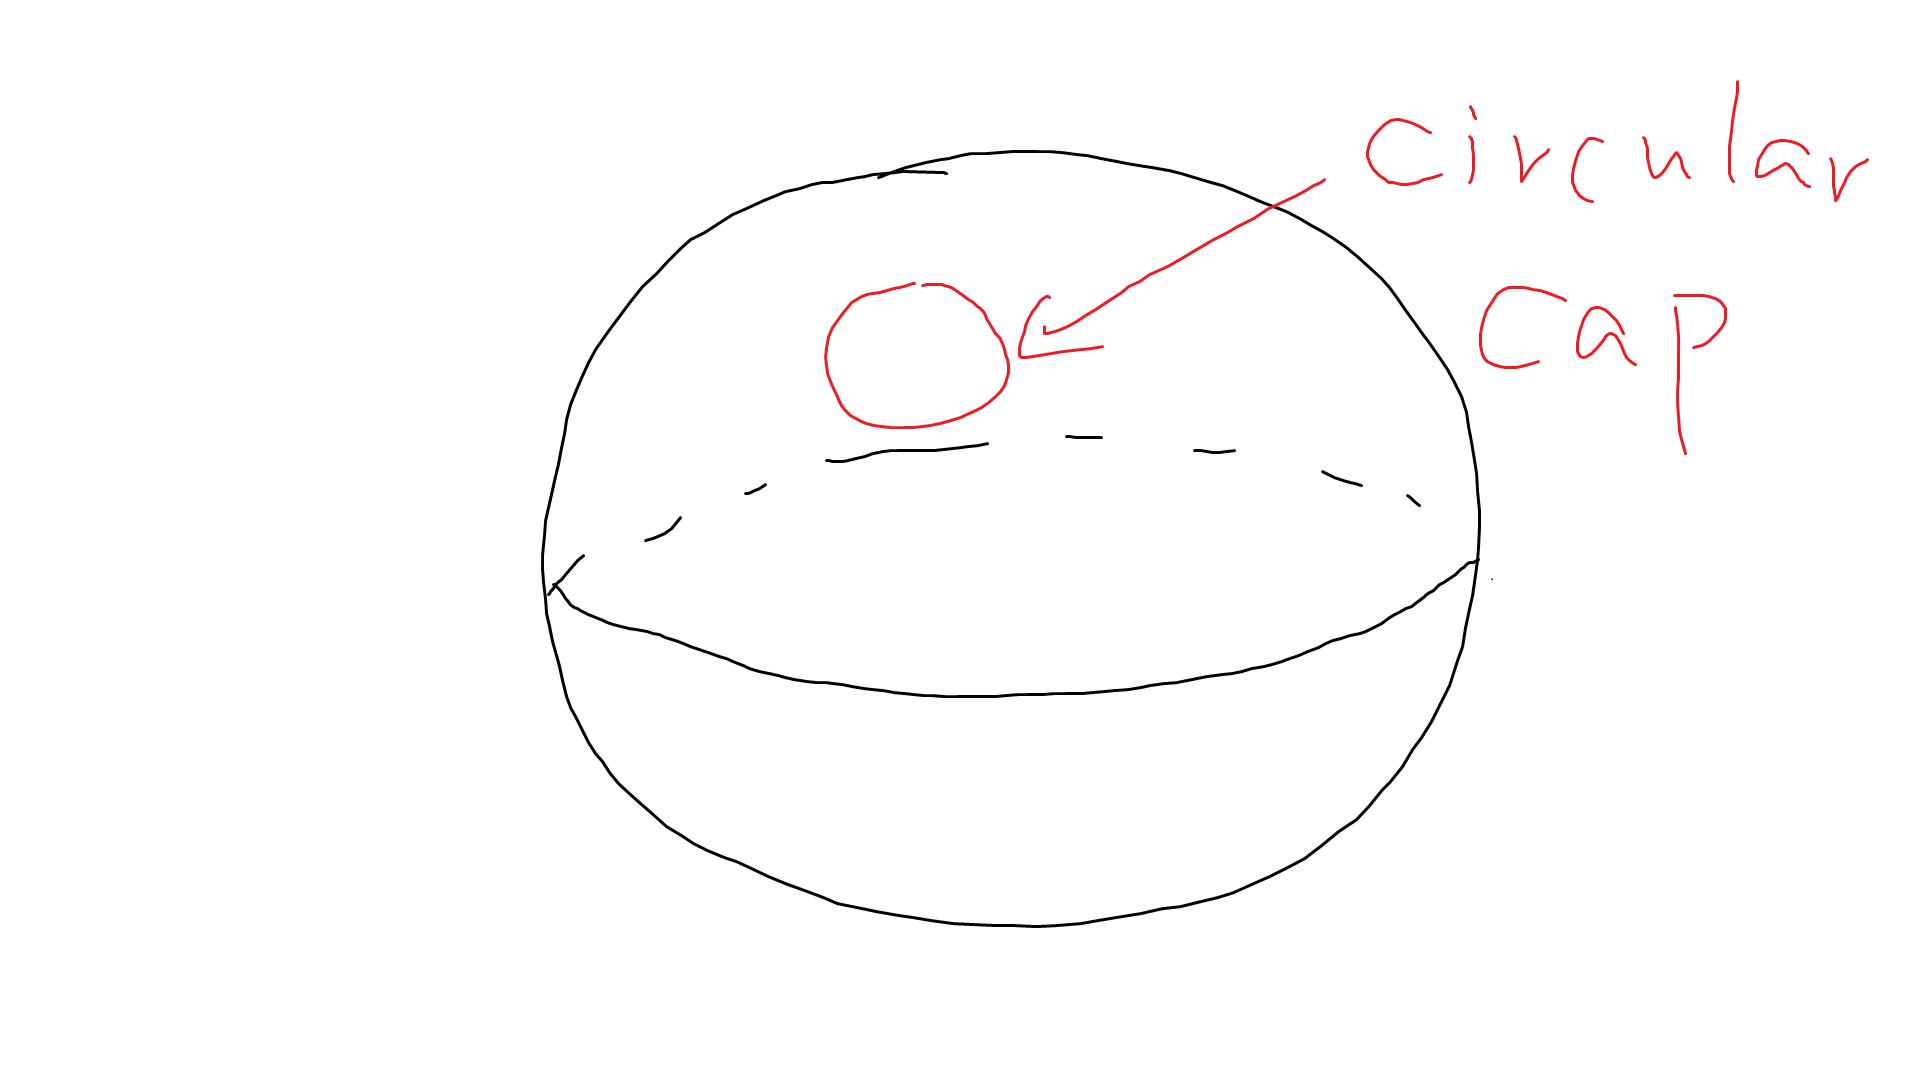
\includegraphics[scale=0.5]{image/Comb_01.png}

For a set $A$ of vertices in a graph $G$, the \emph{boundary} of $A$ is $b(A) = \{x\in V(G): x \not\in A, xy \in E$ for some $y \in A\}$.\\
e.g. in diagram
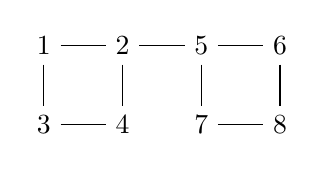
\begin{tikzpicture}
    \node (1) at (0,0) {1};
    \node (2) at (1,0) {2};
    \node (3) at (0,-1) {3};
    \node (4) at (1,-1) {4};
    \node (5) at (2,0) {5};
    \node (6) at (3,0) {6};
    \node (7) at (2,-1) {7};
    \node (8) at (3,-1) {8};

    \path (1) edge (2);
    \path (1) edge (3);
    \path (2) edge (4);
    \path (3) edge (4);
    \path (2) edge (5);
    \path (5) edge (6);
    \path (5) edge (7);
    \path (6) edge (8);
    \path (7) edge (8);
\end{tikzpicture}
, if $A = \{1,2,3\}$, then $b(A) = \{4,5\}$.

An \emph{isoperimetric inequality} of $G$ is an inequality of form: $|B(A)| \geq f(|A|) \forall A \subset V(G)$.\\
Equivalently, minimise the \emph{neighbourhood} of $A$: $N(A) = A \cup b(A) = \{x \in G: d(x,A) \leq 1\}$.\\
A natural guess is often $B(x,r) = \{y \in G: d(x,y) \leq r\}$.\\
What happens in $Q_n$? e.g. $|A| = 4$ in $Q_3$, take all vertices with at least one component 0, then $|b(A)| = 3$; if we instead take all vertices in the lower half plane then $|b(A)| = 4$.

Our guess: \emph{balls are best}, i.e. if $|A| = |X^{(\leq r)}|$, then $|N(A)| \geq |X^{(\leq r+1)}|$ (obvious notations).\\
What if $|A|$ is strictly between $\sum_{i=0}^r {n \choose i}$ and $\sum_{i=0}^{r+1} {n \choose i}$?\\
We guess that $A=X^{(\leq r)} \cup B$ for some $B \subset X^{(r+1)}$ (this is called a \emph{hamming ball}).\\
If we knew this, then $N(A) = X^{(\leq r+1)} \cup \partial^+ B$; hence in this case we know which $B$ to take -- by K-K theorem, take $B$ to be an initial segment of \emph{lex}.

We define the \emph{simplicial} order on $Q_n$ by $x<y$ if either $|x| < |y|$ or $|x|=|y|$ and $x<y$ in lex.\\
Our aim then becomes proving that initial segments of simplicial are best.\\

Given $A \subset Q_n$, and $1 \leq i \leq n$, the \emph{$i$-section} are the set systems $A^{(i)}_+, A^{(i)}_- \subset \P(X-i)$ (\emph{$Q_{n-1}$}), given by
$$A^{(i)}_- = \{x \in A:i \not\in X \} \subset \P(X-i)$$
$$A^{(i)}_+ = \{x -\{i\}: x \in A, i \in x\} \subset \P(X-i)$$
(the first is taking all elements of $A$ that don't contain $i$, the second is taking all elements of $A$ that have $i$ and then throw $i$ away and keep the result).

Define the \emph{$i$-compression} $C_i(A)$ of $A$ by giving its $i$-sections:\\
$C_i(A)^{(i)}_+ =$ initial segment of $Q_{n-1}$ of size $|A^{(i)}_+|$;
$C_i(A)^{(i)}_- =$ initial segment of $Q_{n-1}$ of size $|A^{(i)}_-|$;

Certainly, $|C_i(A)| = |A|$. Also, $C_i(A)$ \emph{looks more like} an initial segment of simplicial than $A$ did. We say $A$ is \emph{$i$-compreseed} if $C_i(A) = A$.

\begin{thm} (1, Harper\footnote{Harper first gave a proof with a \emph{lot} of holes inside with no one knowing how to fill those...}'s)\\
    Let $A \subset Q_n$, and let $C$ be the initial segment of simplicial order with $|C| = |A|$. Then $|N(A)| \geq |N(C)|$.\\
    In particular, if $|A| \geq \sum_{i=0}^r {n \choose i}$, then $|N(A)| \geq \sum_{i=0}^{r+1} {n \choose i}$.

    \begin{rem}
        $\bullet$ If we know $A$ is a Hamming ball then we're done by K-K theorem;\\
        $\bullet$ Harper implies K-K trivially: given $B \subset X^{(r)}$, just apply Harper to $A=B \cup X^{(\leq r-1)}$.
    \end{rem}
    
    \begin{proof}
        Induction on $n$. $n=1$ is trivial.\\
        Given $A \subset Q_n(n>1)$: fix $1 \leq i \leq n$. We claim that $|N(C_i(A))| \leq |N(A)|$.\\
        Proof of claim: write $B = C_i(A)$. We have $|N(A)| = |A_+ \cup N(A_-)| + |A_- \cup N(A_+)|$ (downstairs and upstairs respectively. Think)\\
        Similarly, $|N(B)| = |B_+ \cup N(B_-)| + |B_- \cup N(B_+)|$.\\
        Now $|B_+| = |A_+|$, and $|N(B_-)| \leq |N(A_-)|$ (induction). But $N(B_-)$ is an initial segment of simplicial (on $Q_{n-1}$), as is $B_+$, so $N(B_-)$ and $B_+$ are \emph{nested} (i.e. one belongs to another).\\
        Hence $|B_+ \cup N(B_-)| \leq |A_+ \cup N(A_-)|$.\\
        Similarly, $|B_- \cup N(B_+)| \leq |A_- \cup N(A_+)|$. Thus $|N(B)| \leq |N(A)|$.\\

        ---Lecture 8---

        Among all $B \subset Q_n$ with $|B| = |A|$ and $|N(B)| \leq |N(A)|$, choose one with $\sum_{x \in B} f(x)$ minimal where $f(x)$ is the position of $x$ in simplicial order on $Q_n$. Then $B$ is $i$-compressed $\forall i$.\\
        Must such $A,B$ be an initial segment of simplicial? Unfortunately the answer is no, e.g. take $A=\{\phi,1,2,12\} \subset Q_3$.
        However we have 
        \begin{lemma} (2)\\
            Let $B \subset Q_n$ be $i$-compressed for all $i$, but not an initial segment of the simplicial order. Then\\
            $\bullet$ If $n=2k+1$ is odd, we have $B=X^{(\leq k)} - (k+2)(k+3)...(2k)(2k+1) \cup 12...k(k+1)$, i.e. removing the last element in $X^{(k)}$ but add in the first element in $X^{(k+1)}$;\\
            $\bullet$ If $n=2k$ is even, we have $B=X^{(\leq k-1)} \cup \{x \in X^{(k)}: 1 \in x\} - 1(k+2)(k+3)...(2k) \cup 234...k(k+1)$, i.e. cut exactly half in the middle layer but removing the last element with 1 and add in the first element without 1.

            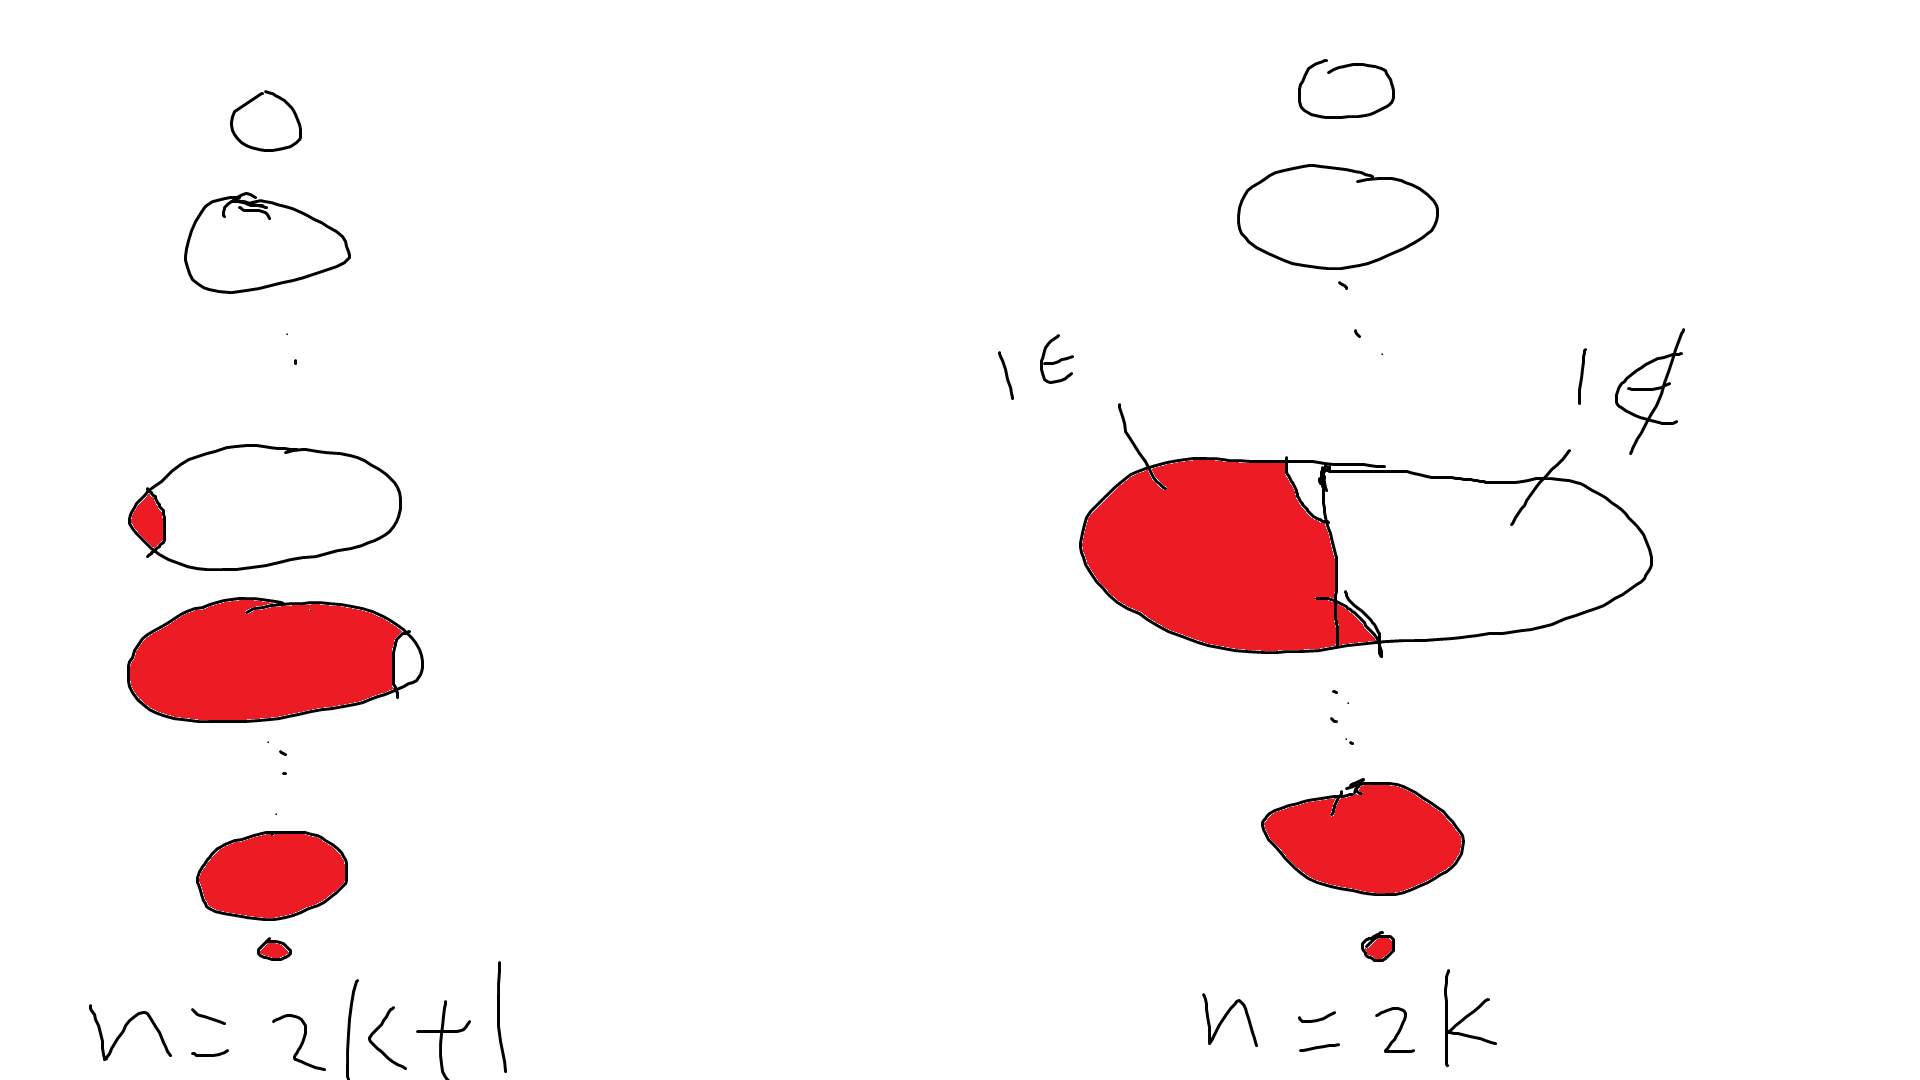
\includegraphics[scale=0.5]{image/Comb_02.png}

            Note that this is trivially beaten by the initial segment of the same size -- so we can prove Harper's theorem if we could prove this.
            \begin{proof}
                Suppose we have $x \not\in B, y \in B$ for some $x,y$ with $x<y$ in simplicial order. Note that we cannot have $i \in x, i \in y$ (as $B$ is $i$-compressed) for any $i$; similarly we cannot have $i \not\in x, i \not\in y$. So $x$ and $y$ must be complement to each other.\\
                Hence for each $y \in B$, at most one $x<y$ has $x \not\in B$ (namely $y^c$); and for each $x\not\in B$ at most one $y>x$ ahs $y \in B$ ($x^c$). Hence $B=\{z:z \leq y\} - \{x\}$, where $x$ is the immediate predecessor of $y$ and $x=y^c$. But then $x$ is the last $k$-set (if $n=2k+1$) or the last $k$-set containing 1 (if $n=2k$).
            \end{proof}
        \end{lemma}
    \end{proof}
\end{thm}

\begin{rem}
    1. We can also prove this by $UV$-compressions.\\
    2. We can also use these \emph{codimension-1} compression to prove K-K theorem directly.
\end{rem}

Now there's no reason to consider only the neighbourhood within one step. For $A \subset Q_n$, the \emph{$t$-neighbourhood} of $A$ is $A_{(t)} = N^t (A) = \{x \in Q_n: d(x,A) \leq t\}$.

\begin{coro} (3)\\
    Let $A \subset Q_n$ with $|A| = |X^{(\leq r)}|$. Then, for $1 \leq t \leq n-r$, we have $|A_{(t)}| \geq |X^{(\leq r+t)}|$.
    \begin{proof}
        Apply Harper's theorem and use induction.
    \end{proof}
\end{coro}

To get a feel for what corollary 3 is saying, we'll need some estimates on things like $\sum_{i=0}^r {n\choose i}$. Note that this is essentially just estimating $\P(X<=r)$ where $X \sim B(n,\frac{1}{2})$. So by CLT we could just use normal distribution to get an accurate estimate when $n$ is large.\\
Lecturer decided to still write a proposition down in the end.

\begin{prop} (4)\\
    Let $0 < \varepsilon < \frac{1}{4}$, Then for $r=\lfloor \frac{1}{2} -\varepsilon/n\rfloor$, the above sum (let's use $S$ to denote that) is at most $\frac{1}{\varepsilon} e^{-\varepsilon^2 n/2} 2^n$ (an exponentially small fraction of $2^n$, with $\varepsilon$ fixed).\\
    \begin{proof}
        For $i \leq (\frac{1}{2} - \varepsilon) n$:
        \begin{equation*}
            \begin{aligned}
                \frac{{n \choose {i-1}}}{{n \choose i}} &= \frac{i}{n-i+1} \leq \frac{\frac{1}{2}-\varepsilon}{\frac{1}{2}+\varepsilon}\\
                &= 1-\frac{2\varepsilon}{\frac{1}{2}+\varepsilon}\\
                &\leq 1-2\varepsilon
            \end{aligned}
        \end{equation*}
        Hence $S \leq \frac{1}{2\varepsilon}{n \choose {\lfloor (\frac{1}{2}-\varepsilon) n \rfloor}}$.\\
        Similarly we could estimate (note we have to be careful about the floor sign)
        \begin{equation*}
            \begin{aligned}
                {n \choose {\lfloor (\frac{1}{2}-\varepsilon) n \rfloor}} &\leq (1-\varepsilon)^{\varepsilon n/2-1} {n \choose {\lfloor (\frac{1}{2}-\frac{\varepsilon}{2}) n \rfloor}}\\
                &\leq 2(1-\varepsilon)^{\varepsilon n/2} 2^n\\
                &\leq 2 e^{-\varepsilon \cdot \varepsilon n/2} \cdot 2^n
            \end{aligned}
        \end{equation*}
        Thus $S \leq \frac{1}{2\varepsilon} 2e^{-\varepsilon^2 n/2} 2^n$.
    \end{proof}
\end{prop}

\end{document}
